\documentclass[11pt,twocolumn,twoside]{article}


\providecommand{\tightlist}{%
  \setlength{\itemsep}{0pt}\setlength{\parskip}{0pt}}\usepackage{longtable,booktabs,array}
\usepackage{calc} % for calculating minipage widths
% Correct order of tables after \paragraph or \subparagraph
\usepackage{etoolbox}
\makeatletter
\patchcmd\longtable{\par}{\if@noskipsec\mbox{}\fi\par}{}{}
\makeatother
% Allow footnotes in longtable head/foot
\IfFileExists{footnotehyper.sty}{\usepackage{footnotehyper}}{\usepackage{footnote}}
\makesavenoteenv{longtable}
\usepackage{graphicx}
\makeatletter
\def\maxwidth{\ifdim\Gin@nat@width>\linewidth\linewidth\else\Gin@nat@width\fi}
\def\maxheight{\ifdim\Gin@nat@height>\textheight\textheight\else\Gin@nat@height\fi}
\makeatother
% Scale images if necessary, so that they will not overflow the page
% margins by default, and it is still possible to overwrite the defaults
% using explicit options in \includegraphics[width, height, ...]{}
\setkeys{Gin}{width=\maxwidth,height=\maxheight,keepaspectratio}
% Set default figure placement to htbp
\makeatletter
\def\fps@figure{htbp}
\makeatother

\usepackage{float}
\makeatletter
\let\oldlt\longtable
\let\endoldlt\endlongtable
\def\longtable{\@ifnextchar[\longtable@i \longtable@ii}
\def\longtable@i[#1]{\begin{figure}[H]
\onecolumn
\begin{minipage}{0.5\textwidth}
\oldlt[#1]
}
\def\longtable@ii{\begin{figure}[H]
\onecolumn
\begin{minipage}{0.5\textwidth}
\oldlt
}
\def\endlongtable{\endoldlt
\end{minipage}
\twocolumn
\end{figure}}
\makeatother
\usepackage{iccr2024}
\usepackage{newtxtext,newtxmath}
\makeatletter
\@ifpackageloaded{caption}{}{\usepackage{caption}}
\AtBeginDocument{%
\ifdefined\contentsname
  \renewcommand*\contentsname{Table of contents}
\else
  \newcommand\contentsname{Table of contents}
\fi
\ifdefined\listfigurename
  \renewcommand*\listfigurename{List of Figures}
\else
  \newcommand\listfigurename{List of Figures}
\fi
\ifdefined\listtablename
  \renewcommand*\listtablename{List of Tables}
\else
  \newcommand\listtablename{List of Tables}
\fi
\ifdefined\figurename
  \renewcommand*\figurename{Figure}
\else
  \newcommand\figurename{Figure}
\fi
\ifdefined\tablename
  \renewcommand*\tablename{Table}
\else
  \newcommand\tablename{Table}
\fi
}
\@ifpackageloaded{float}{}{\usepackage{float}}
\floatstyle{ruled}
\@ifundefined{c@chapter}{\newfloat{codelisting}{h}{lop}}{\newfloat{codelisting}{h}{lop}[chapter]}
\floatname{codelisting}{Listing}
\newcommand*\listoflistings{\listof{codelisting}{List of Listings}}
\makeatother
\makeatletter
\makeatother
\makeatletter
\@ifpackageloaded{caption}{}{\usepackage{caption}}
\@ifpackageloaded{subcaption}{}{\usepackage{subcaption}}
\makeatother

\addbibresource{../references.bib}
\title{A mixture of hidden Markov models to predict the lymphatic spread
in head and neck cancer depending on primary tumor location}

\author[%
1,2%
]{Roman Ludwig}
\author[%
1,2%
]{Julian Brönnimann}
\author[%
1,2%
]{Yoel Pérez Haas}
\author[%
1,2%
]{Esmée Lauren Looman}
\author[%
2%
]{Panagiotis Balermpas}
\author[%
11%
]{Sergi Benavente}
\author[%
3,4,7%
]{Adrian Schubert}
\author[%
8%
]{Dorothea Barbatei}
\author[%
8%
]{Laurence Bauwens}
\author[%
2%
]{Jean-Marc Hoffmann}
\author[%
3%
]{Olgun Elicin}
\author[%
6,10%
]{Matthias Dettmer}
\author[%
2%
]{Bertrand Pouymayou}
\author[%
4,5%
]{Roland Giger}
\author[%
8%
]{Vincent Grégoire}
\author[%
1,2%
]{Jan Unkelbach}

\affil[1]{Department of Physics, %
University of Zurich%
, Zurich%
%
%
, Switzerland}
\affil[2]{Department of Radiation Oncology, %
University Hospital Zurich%
, Zurich%
%
%
, Switzerland}
\affil[3]{Department of Radiation Oncology, %
Bern University Hospital%
, Bern%
%
%
, Switzerland}
\affil[4]{Department of ENT, Head \& Neck Surgery, %
Bern University Hospital%
, Bern%
%
%
, Switzerland}
\affil[5]{Head and Neck Anticancer Center, %
Bern University Hospital%
, Bern%
%
%
, Switzerland}
\affil[6]{Institute of Tissue Medicine and Pathology, %
Bern University Hospital%
, Bern%
%
%
, Switzerland}
\affil[7]{Department of ENT, Head \& Neck Surgery, %
Réseau Hospitalier Neuchâtelois%
, Neuchâtelois%
%
%
, Switzerland}
\affil[8]{Department of Radiation Oncology, %
Centre Léon Bérard%
, Lyon%
%
%
, France}
\affil[9]{Department of Head and Neck Surgery, %
Centre Léon Bérard%
, Lyon%
%
%
, France}
\affil[10]{Institute of Pathology, %
Klinikum Stuttgart%
, Stuttgart%
%
%
, Germany}
\affil[11]{Departement of Radiation Oncology, %
Hospital Vall d'Hebron%
, Barcelona%
%
%
, Spain}

\date{}
\begin{document}

\maketitle
\thispagestyle{fancy}

\begin{customabstract}
We previously developed a mechanistic hidden Markov model (HMM) to
predict the lymphatic tumor progression in oropharyngeal squamous cell
carcinomas. To extend the model to other tumor subsites in the head and
neck defined by ICD-10 codes, we develop a mixture model combining
multiple HMMs. The mixture coefficients and the model parameters are
learned via an EM-like algorithm from a large multi-centric dataset on
lymph node involvement. The methodology is demonstrated for tumors in
the oropharynx and oral cavity. The mixture model groups anatomically
nearly subsites and yields interpretable mixture coefficients consistent
with anatomical location. It allows the prediction of differences in
lymph node involvement depending on tumor subsite.
\end{customabstract}



\section{Introduction}\label{introduction}

Head and neck squamous cell carcinomas (HNSCC) frequently spread through
the lymphatic system
\autocite{lindberg_distribution_1972,woolgar_histological_1999}. Current
diagnostic imaging modalities are unable to detect microscopic lymph
node metastases \autocite{snyder_petct_2021,strohl_petct_2021}. To avoid
nodal recurrences, large volumes in the neck, which are at risk of
harbouring occult disease, are irradiated electively. Guidelines about
which lymph node levels (LNLs) to irradiate
\autocite{biau_selection_2019} are currently not based on a patient's
individual risk, but on the overall prevalence of nodal disease as
reported in the literature
\autocite{lindberg_distribution_1972,woolgar_histological_1999}.

To personalize the prediction of the risk for occult disease, given a
patient's individual diagnosis, we published

\begin{enumerate}
\def\labelenumi{\arabic{enumi}.}
\tightlist
\item
  large, multi-centric data that reports per patient which LNLs were
  clinically/pathologically involved
  \autocite{ludwig_dataset_2022,ludwig_multi-centric_2023}.
\end{enumerate}

And, building on this work,

\begin{enumerate}
\def\labelenumi{\arabic{enumi}.}
\setcounter{enumi}{1}
\tightlist
\item
  an interpretable hidden Markov model (HMM), trained with this data, to
  predict the risk for occult nodal disease, given an individual
  patient's diagnosis \autocite{ludwig_hidden_2021}.
\end{enumerate}

Such a personalized risk prediction may allow clinicians to safely
reduce the elective clinical target volume (CTV-N) and thus reduce
side-effects that degrade the patient's quality of life without
compromising treatment efficacy \autocite{batth_practical_2014}.

Here, we extend the previous work by incorporating the primary tumor
location (specified as ICD-10 code) into the model of lymphatic tumor
progression, focusing on tumors in the oropharynx and the oral cavity.
HNSCC patients with primary tumors at different subsites show different
patterns of lymphatic spread
\autocite{lindberg_distribution_1972,woolgar_histological_1999}. So far,
this could be handled by training different models for broader
categories of tumor locations, e.g.~oropharynx and oral cavity tumors.
However, this approach does not describe differences in lymphatic spread
between different subsites within the oropharynx and oral cavity. To
address this issue, we present an approach using mixtures of HMMs. The
intuition is that the lymphatic spread of a tumor that lies anatomically
at the boarder of oropharynx and oral cavity (e.g.~tumors in the palate)
may be described by a mixture of different models. Tumor subsites used
in this work are sketched in figure~\ref{fig-schematic-and-graph}.

\section{Materials and Methods}\label{sec-materials-and-methods}

Each LNL \(v \in \{ 1, 2, \ldots, V\}\) considered in our model is
represented by a binary random variable \(X_v\) representing the true
state of that level (0 for ``healthy'' and 1 for ``involved''). A
patient's state of lymph node involvement can be represented in a random
vector \(\mathbf{X} = \left( X_1, X_2, \ldots, X_V \right)\). When a
patient is diagnosed with HNSCC, we only observe the clinical lymph node
involvement based on imaging, which we denote as another binary random
variable \(Y_v\). To compute the personalized risk of occult disease
\(\mathbf{X}\), given a diagnosis \(\mathbf{Y}\), we apply Bayes' law:

\begin{equation}\phantomsection\label{eq-bayes-law}{
P \left( \mathbf{X} \mid \mathbf{Y} \right) = \frac{P \left( \mathbf{Y} \mid \mathbf{X} \right) P \left( \mathbf{X} \right)}{\sum_{\mathbf{X}^\star} P \left( \mathbf{Y} \mid \mathbf{X}^\star \right) P \left( \mathbf{X}^\star \right)}
}\end{equation}

In the above equation, the term
\(P \left( \mathbf{Y} \mid \mathbf{X} \right)\) is given by the
sensitivity and specificity of the diagnostic procedure. The term
\(P \left( \mathbf{X} \right)\) represents the prior probability of
involvement, which depends on the probability of the tumor to spread
through the lymphatic system. The main task of the HMM is to model
\(P \left( \mathbf{X} \right)\) and the main contribution of this paper
is to incorporate the primary tumor subsite into the model of
\(P \left( \mathbf{X} \right)\).

\subsection{Hidden Markov Model for Lymphatic
Progression}\label{sec-hmm}

A patient's state of lymph node involvement \(\mathbf{X}[t]\) evolves
over discrete time steps \(t\). Let us enumerate all \(2^V\) possible
states, representing all combinations of LNLs. In this paper, we
consider ipsilateral LNLs I, II, III and IV, which amounts to 16
possible states. The HMM is specified by a \emph{transition matrix}:

\begin{equation}\phantomsection\label{eq-transition-matrix}{
\mathbf{A} = \begin{pmatrix} A_{ij} \end{pmatrix} = P \left( \mathbf{X}[t+1] = \boldsymbol{\xi}_j \mid \mathbf{X}[t] = \boldsymbol{\xi}_i \right)
}\end{equation}

whose elements \(A_{ij}\) contain the conditional probabilities that a
state \(\mathbf{X}[t]=\boldsymbol{\xi}_i\) transitions to
\(\mathbf{X}[t+1]=\boldsymbol{\xi}_j\) over one time step. The
transition matrix is specified and parameterised via the graphical model
shown in figure~\ref{fig-schematic-and-graph}. The red arcs in the graph
of figure~\ref{fig-schematic-and-graph} (right panel) are associated
with the probability that the primary tumor spreads directly to a LNL
(parameters \(b_v\)). The blue arcs describe the spread from an upstream
LNL -- given it is already metastatic -- to a downstream level
(parameters \(t_{v \rightarrow v+1}\)).

Now, let \(\boldsymbol{\pi}\) be the \emph{starting distribution}

\begin{equation}\phantomsection\label{eq-starting-distribution}{
\boldsymbol{\pi} = \begin{pmatrix} \pi_i \end{pmatrix} = P \left( \mathbf{X}[0] = \boldsymbol{\xi}_i \right)
}\end{equation}

denoting the probability to start in state \(\boldsymbol{\xi}_i\) at
time step 0. Assuming that every patient started with all LNLs being
healthy, we set \(\pi_i\) to zero for all states except the completly
healthy state
\(\boldsymbol{\xi} = \begin{pmatrix} 0, 0, 0, 0 \end{pmatrix}\), which
has probability one.

Using the quantities introduced so far, the probability
\(P \left( \mathbf{X}[t]=\boldsymbol{\xi}_i \right)\) to be in state
\(\boldsymbol{\theta}_i\) in time step \(t\) can now be conveniently
expressed as a matrix product:

\begin{equation}\phantomsection\label{eq-evolution}{
P \left( \mathbf{X}[t]=\boldsymbol{\xi}_i \right) = \left( \boldsymbol{\pi} \cdot \mathbf{A}^t \right)_i
}\end{equation}

This evolution implicitly marginalizes over all possible paths to arrive
at state \(\boldsymbol{\xi}_i\) after \(t\) time-steps. Additionally, we
must marginalize over the unknown time of diagnosis using a time-prior
\(P_T(t)\). This finally defines the probability distribution over all
states of lymph node involvement used in equation~\ref{eq-bayes-law}.

\begin{equation}\phantomsection\label{eq-marginalized-evolution}{
P \left( \mathbf{X}=\boldsymbol{\xi}_i \mid \boldsymbol{\theta} \right) = \sum_{t=0}^{t_\text{max}} P_T(t) \left( \boldsymbol{\pi} \cdot \mathbf{A}^t \right)_i
}\end{equation}

where \(\boldsymbol{\theta}=\{ b_v, t_{v \rightarrow v+1} \}\) denotes
the set of all model parameters (7 in our case). Fortunately, the exact
length and shape of this distribution has little impact as previously
shown \autocite{ludwig_hidden_2021}. We set \(t_\text{max}=\) 10 and
\(P_\text{early}(t)\) to a binomial distribution with parameter 0.3.
Further details on the HMM can be found in \textcite{ludwig_hidden_2021}
and \textcite{zora231470}.

\begin{figure}[th]

\centering{

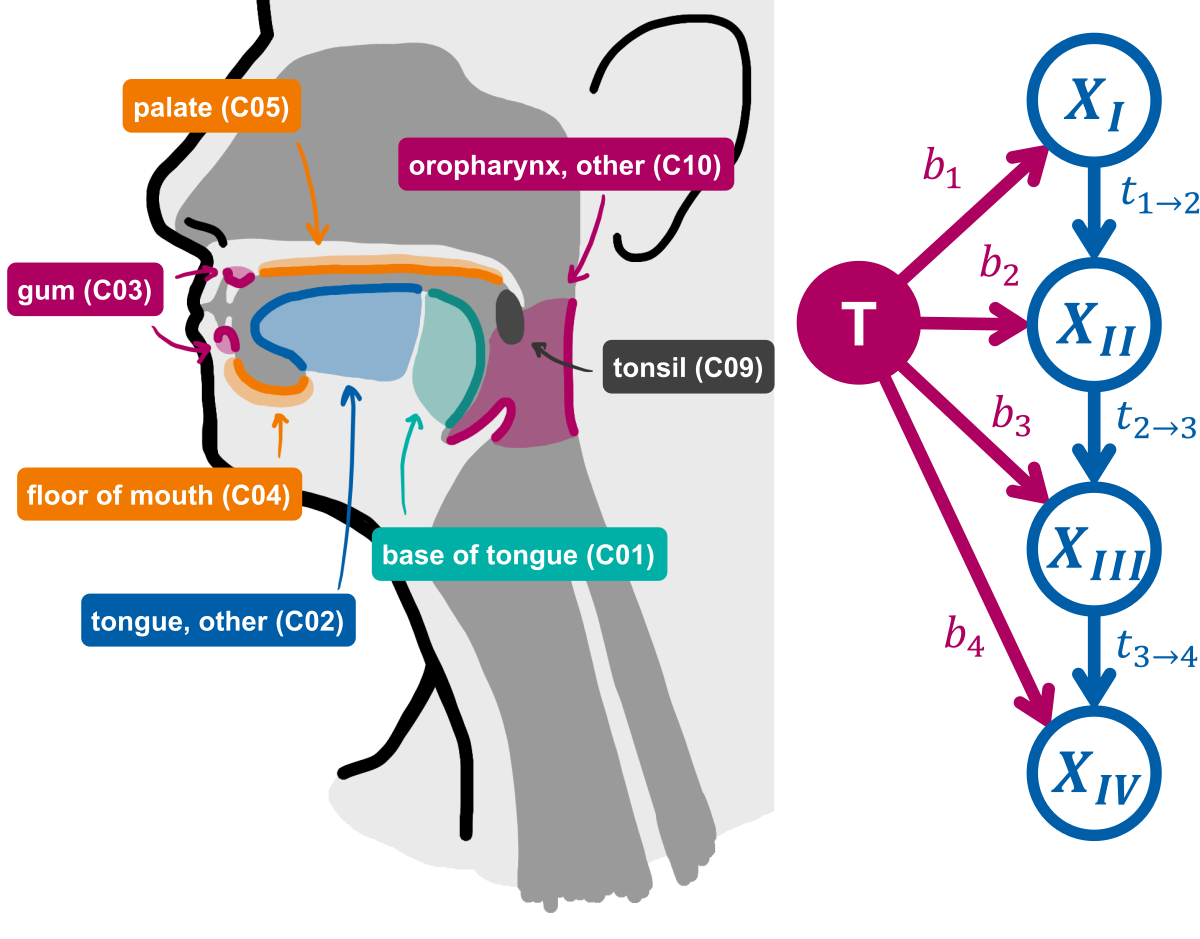
\includegraphics{../static/schematic_and_graph.png}

}

\caption{\label{fig-schematic-and-graph}On the left: Anatomical sketch
of the tumor subsites and corresponding ICD-10 codes considered in this
work. The subsite ``other parts of mouth'' (C06) was not drawn. On the
right: Parametrized graphical model of the lymphatic network considering
four LNLs. Blue nodes represent the hidden states of LNLs \(X_v\), while
the red one is the tumor. Arcs represent possible routes of metastatic
spread, associated with a probability.}

\end{figure}%

\subsection{Mixture of HMMs}\label{sec-mixture-of-hmms}

Let us now assume that primary tumors at different subsites have
different patterns of lymphatic spread, corresponding to different model
parameters \(\boldsymbol{\theta}\). Training a separate model for every
possible subsite (ICD-10 code) would require a sufficiently large
dataset for every tumor site. However, anatomically nearby locations are
expected to show very similar patterns of LNL involvement. Therefore, we
consider a mixture model.

Let us assume that we have a dataset \(\mathbf{D}\) that is specified
via the number of patients \(N_{is}\) that were diagnosed in LNL
involvement state \(i\) and had a primary tutor in subsite \(s\). Let us
further assume that we want to describe this dataset using a mixture of
\(M\) HMMs, each with a different set of model parameters
\(\boldsymbol{\theta_m}\). As the generative model of the data, we
assume that a patient with subsite \(s\) is generated with probability
\(\pi_{sm}\) from model \(m\). The likelihood of the dataset can then be
written as

\begin{equation}\phantomsection\label{eq-mixture-distribution}{
P \left( \mathbf{D} \mid \boldsymbol{\theta}, \boldsymbol{\pi}\right) = \prod_s \prod_i \left[ \sum_{m=1}^M \pi_{sm} P_m \left( \mathbf{X}=\boldsymbol{\xi}_i \mid \boldsymbol{\theta}_m \right) \right]^{N_{is}}
}\end{equation}

We now have two types of parameters, the probabilities of tumor spread
for the different models, \(\boldsymbol{\theta_m}\), and the mixing
coefficients \(\pi_{sm}\). Assuming a uniform prior in the interval
\([0,1]\) for all parameters, the posterior distribution over the
parameters
\(P \left( \boldsymbol{\theta}, \boldsymbol{\pi} \mid \mathbf{D} \right)\)
is given by the likelihood in equation~\ref{eq-mixture-distribution}
except for a normalisation constant. In this work, we use Markov chain
Monte Carlo sampling (MCMC) via the \texttt{emcee} Python package
\autocite{foreman-mackey_emcee_2013} to sample model parameters from the
posterior distribution. However,
\(P \left( \boldsymbol{\theta}, \boldsymbol{\pi} \mid \mathbf{D} \right)\)
itself is a multi-model distribution because one can permute the
different models. To address this problem, we revert to an
\emph{expectation-maximization (EM)} algorithm where we iterate two
steps until convergence of the mixing coefficients. In the E-step, we
sample model parameters \(\boldsymbol{\theta_m}\) using MCMC for given
mixing coefficients \(\pi_{sm}\). In the M-step, we maximize the
likelihood with respect to the mixing coefficients for given samples of
\(\boldsymbol{\theta_m}\)

\subsection{Multi-Centric Data}\label{multi-centric-data}

For the analyses in this work, we used five datasets from four different
institutions, resulting in 1242 patients in total.

\begin{enumerate}
\def\labelenumi{\arabic{enumi}.}
\tightlist
\item
  287 oropharyngeal patients from the University of Zurich in
  Switzerland
\item
  263 oropharyngeal patients from the Centre Léon Bérard in France
\item
  289 oropharyngeal and oral cavity patients from the Inselspital Bern
  in Switzerland
\item
  239 oropharyngeal and oral cavity patients from the Centre Léon Bérard
  in France
\item
  162 oropharyngeal patients from the Hospital Vall d'Hebron in Spain
  (not yet public)
\end{enumerate}

\begin{figure}[b]

\centering{

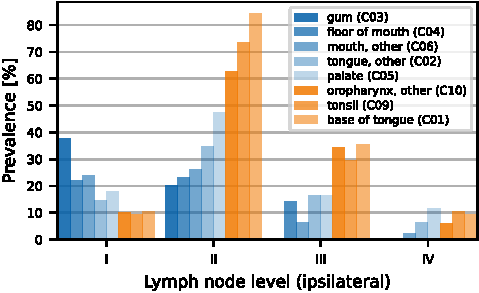
\includegraphics{manuscript_files/mediabag/../figures/prevalence_by_subsite.pdf}

}

\caption{\label{fig-prevalence-by-subsite}Prevalence of ipsilateral LNL
involvement stratified by subsite. The subsites are sorted in ascending
order by their prevalence of involvement in LNL II. Oral cavity subsites
are plotted in shades of blue, oropharynx subsites in shades of orange.}

\end{figure}%

The data sets 1-4 are publicly available in the form of CSV tables
\autocite{ludwig_detailed_2022,ludwig_multi-centric_2023} and may be
interactively explored in our \textbf{Ly}mphatic \textbf{Pro}gression
e\textbf{X}plorer \href{https://lyprox.org}{LyProX}. For each patient,
the primary tumor subsite is reported (among other patient and tumor
characteristics) and each individual LNL is reported as metastatic or
healthy, according to the available diagnostic modalities (in part
pathology after neck dissection, otherwise clinical involvement).

In figure~\ref{fig-prevalence-by-subsite}, we plot the prevalence of
involvement in the four ipsilateral LNLs I, II, III, and IV stratified
by the primary tumor's subsite. The figure illustrates the variations in
LNL involvement between subsites within the oral cavity and oropharynx
categories. The number of patients for each subsite is indicated in
figure~\ref{fig-cluster-assignments}.

\section{Results}\label{sec-results}

We demonstrate the methodology for a mixture model with \(M=2\)
components, considering the ipsilateral involvement of LNLs I, II, III,
and IV and the primary tumor subsites shown in
figure~\ref{fig-prevalence-by-subsite}. In
figure~\ref{fig-cluster-assignments} we show the resulting mixture
coefficients \(\pi_{sm}\). The interpretation of this result is as
follows: tumors of the base of tongue (C01) are fully described by
component A, and tumors of the gum (C03) are fully described by
component B. These two subsites are the most distinct regarding the
involvement of LNLs I and II, and the result is thus intuitive.
Component A may be interpreted as a model for oropharynx-like tumor
spread, and component B as a model for oral cavity-like tumor spread.
All other subsites are described as mixtures. tumors in the tonsil (C09)
have LNL involvement similar to base of tongue tumors and are mostly
assigned to component A. Instead, tumors of the palate (C05) are to
similar degree assigned to components A and B, which is consistent with
the anatomical location and the observation that the LNL involvement is
in between oropharynx and oral cavity-type patterns
(figure~\ref{fig-prevalence-by-subsite}).

\begin{figure}

\centering{

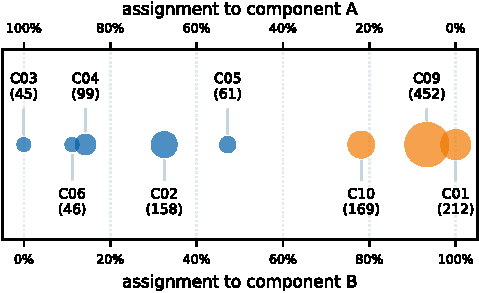
\includegraphics{manuscript_files/mediabag/../figures/cluster_assignments.pdf}

}

\caption{\label{fig-cluster-assignments}Assignment of each subsite to
each of the two components. The further left a subsite, the more it is
assigned to component A, the further right, the more to component B. The
size of the marker (area) corresponds to the number of patients in the
subsite.}

\end{figure}%

The figure~\ref{fig-prevalence-comparison} illustrates the model's
predictions of the overall prevalence of lymph node involvement in LNLs
I, II and III (filled histograms) for selected subsites, obtained by
summing the probabilities of states where the respecive level is
involved. The mixture model is compared to two independent HMM models
trained for oral cavity and oropharynx (by pooling the respective
subsites). The mixture model and the independent oropharynx model
perform similarly for tonsil tumors (C09), which is the largest patient
group, dominating the independent oropharynx model and the component B
in the mixture model. However, the mixture model better predicts the
higher prevalence in level II for base of tongue and palate tumors.

\begin{figure*}

\centering{

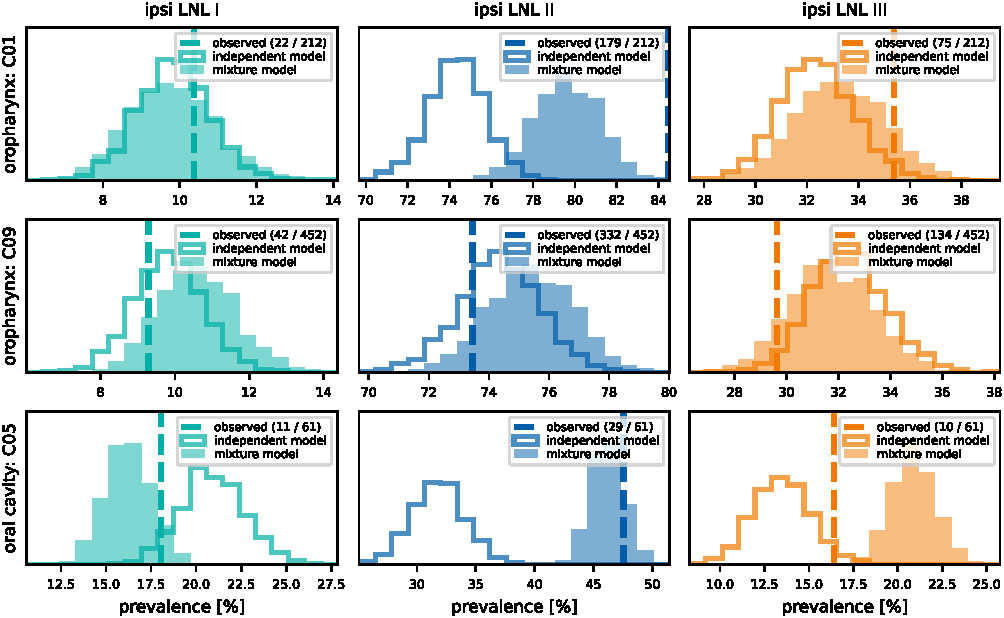
\includegraphics{manuscript_files/mediabag/../figures/prevalence_comparison.pdf}

}

\caption{\label{fig-prevalence-comparison}The prevalence of involvement
as seen in the data (vertical dashed lines), predicted by an independent
model for the oropharyngeal or oral cavity patients (outlined
histograms), and predicted by the mixture model (filled histograms).
Each row correpsonds to one subsite and each column to one LNL.}

\end{figure*}%

\section{Discussion}\label{sec-discussion}

We have previously developed a model of lymphatic progression of HNSCC
using HMM, which allows us to estimate the probability of occult lymph
node metastases in clinically negative LNLs. Mixture models are a
suitable method to incorporate the primary tumor location into the
model, which allows us to account for differences in lymph node
involvement for different subsites. Future work will extend the work to
tumors in the hypopharynx and larynx and optimize the number of model
components.

\section*{Acknowledgements}\label{acknowledgements}
\addcontentsline{toc}{section}{Acknowledgements}

This work was supported by the clinical research priority program (CRPP)
``Artificial intelligence in oncological imaging'' of the University of
Zurich and by the Swiss cancer research foundation under grant KFS
5645--08--2022.

\printbibliography



\end{document}
